\chapter{Aplicação da programação linear na separação de pontos}

Na tarefa onde o obejtivo é a separação de dois ou mais conjuntos de pontos, sendo que cada conjunto representa um padrão, busca-se um método para que essa separação seja obtida com resultado ótimo. Cada conjunto é o resultado de um conjunto de pontos e cada ponto é é representado por um vetor de características.
Em \cite{Bennett92robustlinear} é proposto um modelo de programação linear capaz de um gerar um hiperplano de minimiza a soma dos pontos classificados de forma errada. Dessa forma o modelo é capaz de gerar um hiperplano separador para pontos linearmente separáveis e para conjutnos linearmente inseparáveis, o modelo gera o melhor hiperplano de forma que essa média calculada seja mínima. Na figura abaixo estão ilustrados os casos de dois conjuntos linearmente separáveis e dois conjuntos linearmente inseparáveis. COLOCAR FIGURA!!!
 
\begin{figure}
\centering
\subfigure[]{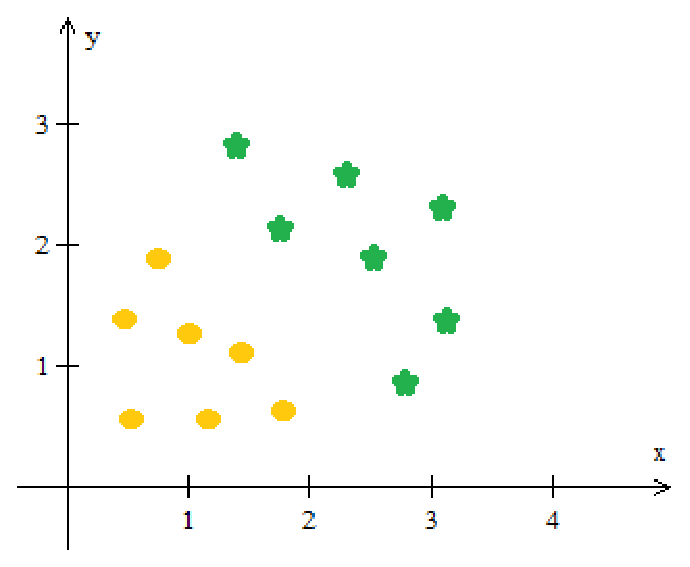
\includegraphics[scale=0.5]{graficos/linear_sepa}\label{fig1}}
\qquad
\subfigure[]{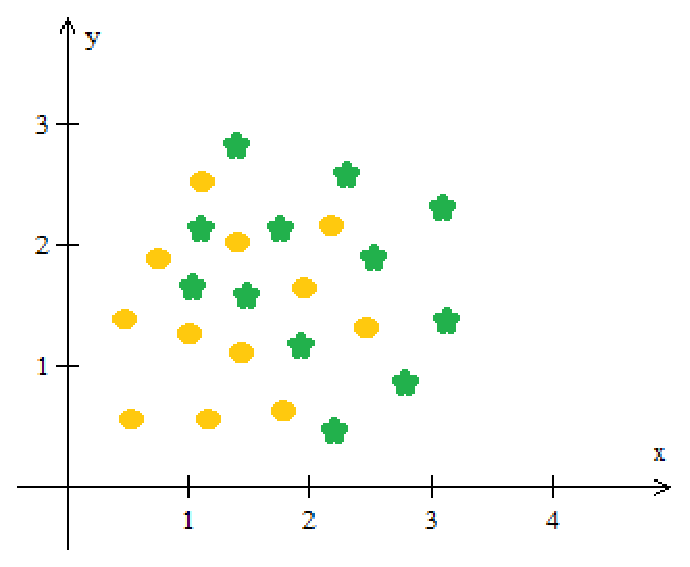
\includegraphics[scale=0.5]{graficos/linear_insepa}\label{fig2}}
\label{img:linear_sepa}
\caption{Em \ref{fig1} são apresentados dois conjuntos linearmente separáveis e em \ref{fig2} são apresentados dois conjuntos linearmente inseparáveis}
\end{figure}

A proposta do modelo e separa dois conjuntos de pontos, porém também pode ser utlizado em problemas onde busca-se a separação de múltiplos padrões. O presente trabalho foca nessa última abordagem, em todos os testes realizados o número de conjutnso de pontos é igual ou maior que três.

\section{O modelo}
Considerando dois conjuntos, no espaço n-dimensional $ R^{n} $, sendo o conjunto A representado pela matriz m x n, e o conjunto B representado pela matriz k x n. Contextualizando, k e m são as quantidades de pontos em cada conjunto, e n é a quantidade de características. O modelo gera um hiperplano que separa os pontos dos dois conjuntos. De forma que os m pontos do conjunto A fiquem de um lado do hiperplano e os k pontos do conjunto B fiquem do outro lado do hiperplano. Na figura abaixo o modelo é apresentado. E a seguir é apresentado de forma mais detalhada.

$$\min_{\omega ,\gamma ,y,z}\frac{e^{T}y}{m}+\frac{e^{T}z}{k}$$
$$s.a.\left\{\begin{matrix}-A\omega +e\gamma+e\leq y\\B\omega -e\gamma+e\leq  z\\ y\geq 0,y\geq 0\end{matrix}\right.$$

O modelo determina o hiperplano:
$$ x\omega = \gamma $$
Onde,  é $\omega$ o vetor normal ao hiperplano e $\gamma$ é um escalar. De forma que:
$$A\omega \geq e\gamma$$
e
$$B\omega \leq e\gamma$$
Onde e é um vetor de 1’s com dimensão m para o conjunto A e k para o conjunto B.
Para conjuntos linearmente separáveis torna-se fácil traçar um hiperplano separador, porém para conjuntos linearmente inseparáveis é necessária uma estratégia para que o hiperplano separador seja ótimo.
O modelo busca o melhor hiperplano, para isso gera dois hiperplanos limites somando 1 unidade a equação do hiperplano separador:
$$A\omega \geq e\gamma + e$$
e
$$B\omega \leq e\gamma - e$$
De forma que o hiperplano separador fica localizado exatamente entre esses dois hiperplanos limites.
Detalhando o modelo de acordo com \citeonline{Eberson10LPseparaPontos}, considerando x como um vetor em $ R^{n} $, definimos:

$1.\ \ (x_{i})_{+} = \max_{i=1,2,...,n}{\left \{x_{i},0  \right \}}$

$2.\ \ \left \| x \right \|_{1} = \sum_{i=1}^{n}\left | x_{i} \right |$

Podemos escrever o problema de minimização com norma da seguinte forma:

$$\min_{\omega ,\gamma }\frac{1}{m}\left \| \left ( -A\omega + e\gamma  + e \right )_{+} \right \|_{1} + \frac{1}{k}\left \| \left ( B\omega - e\gamma + e  \right )_{+} \right \|_{1}$$

Seja $g:R^{n} \mapsto R^{m} , h:R^{n} \mapsto R^{k}$ e S um subconjunto de $R^{n}$ . Os problemas abaixo possuem soluções idênticas:

$$\min_{x\in S}\left \| g(x)_{+} \right \|_{1} + \left \| h(x)_{+} \right \|_{1}$$


$$\min_{x\in S} e^{t}y + e^{t}z\\$$
$$ s.a.\left\{\begin{matrix}y\geq g(x)\\ \geq h(x)\\ y\geq 0, z\geq0\end{matrix}\right.$$

Como $g(x)_{+}\geq g(x)$ e $h(x)_{+}\geq h(x)$ podemos observar que os valores ótimos de y e z podem der dados pelas igualdades $y=g(x)_{+}$ e $z=h(x)_{+}$.

NUMERAR AS EQUAÇÕES!!!
$$\min_{\omega ,\gamma ,y,z}\frac{e^{T}y}{m}+\frac{e^{T}z}{k}$$
$$s.a.\left\{\begin{matrix}-A\omega +e\gamma+e\leq y\\B\omega -e\gamma+e\leq  z\\ y\geq 0,y\geq 0\end{matrix}\right.$$

\underline{Dados do Modelo}:

m: quantidade de imagens no conjunto correspondente a primeira expressão facial;
k: quantidade de imagens no conjunto correspondente a segunda expressão facial;
A: Matriz contendo o conjunto de vetores de caraterísticas das imagens correspondentes à primeira expressão facial;
B: Matriz contendo o conjunto de vetores de caraterísticas das imagens correspondentes à segunda expressão facial;
e:  vetor coluna unitário;

\underline{Variáveis do Modelo}:

$\omega$: coeficientes do hiperplano que separa os conjuntos de imagens em dois grupos;
$\gamma$: constante do hiperplano que separa os conjuntos de imagens em dois grupos;
y: vetor contendo as distâncias de cada imagem do conjunto A ao hiperplano separador mais um;
z: vetor contendo as distâncias de cada imagem do conjunto B ao hiperplano separador mais um.

\underline{Formulação Matemática}:

	A função objetivo (1) procura minimizar a somas das médias das distâncias das imagens de ambos conjuntos. A restrição (2) exige que os pontos se encontrem necessariamente abaixo do hiperplano separador mais uma constante unitária.  A restrição (3) é análoga a restrição (2) aplicada as imagens da segunda expressão facial. As equações em (4) definem a natureza das variáveis do modelo, como sendo não negativas.

\section{Exemplo Ilustrativo do Modelo Classificador}
Para ilustrar o modelo vamos considerar dois exemplos em $R^{2}$ \cite{Bennett92robustlinear} desta que a ilustração gráfica fique mais facilmente compreensível.
\begin{itemize}
\item Exemplo1:

Considerando as matrizes a seguir:
$$A=\begin{bmatrix}1 & 1\\ 1 & 2\\ 1 & 3\\ 2 & 1\\ 2 & 2\\ 2 & 3\\ 2 & 4\\ 3 & 3\\ 3 & 4\end{bmatrix}
B=\begin{bmatrix}4 & 1\\ 4 & 2\\ 4 & 3\\ 5 & 2\\ 5 & 3\\ 5 & 4\\ 6 & 2\end{bmatrix}$$

Nesse caso, temos: m = 9 (quantidade de pontos da matriz A) e k = 7 (quantidade de pontos da matriz B).  Submetendo as matrizes ao modelo temos:
\begin{itemize}
\item[$\ast$] Valor da função objetivo = 0
\item[$\ast$] $\omega$ = [-2  1]
\item[$\ast$] $\gamma$ = -4
\item[$\ast$] y = [0 0 0 0 0 0 0 0 0]
\item[$\ast$] z = [0 0 0 0 0 0 0]
\end{itemize}
Como o valor da função objetivo depende dos vetores y e z, podemos notar que o valor 0 indica que os conjuntos A e B são linearmente separáveis. A seguir é apresentada a representação gráfica dos pontos e das retas geradas pelo modelo.

COLOCAR FIGURA!!!

A partir da representação gráfica podemos perceber que a reta separadora $-2x + y = -4$ se localizou exatamente no meio entre os dois conjuntos com o auxílio das duas retas: $-2x + y = -3$ e $-2x + y = -5$.

\item Exemplo2:
Vamos  considerar agora as matrizes:
$$A=\begin{bmatrix}3 & 4\\ 4.3 & 4.5\\ 4.5 & 2\\ 3 & 5.5\end{bmatrix}
B=\begin{bmatrix}4 & 2\\ 4.5 & 3.5\\ 5 & 3\end{bmatrix}$$

Neste exemplo temos: m = 4 e k = 3. De acordo com o modelo, temos os seguintes valores:
\begin{itemize}
\item[$\ast$] Valor da função objetivo = 0.92
\item[$\ast$] $\omega$ = [-0.91  0.91]
\item[$\ast$] $\gamma$ = -0.82
\item[$\ast$] y = [0 0 2.46 0]
\item[$\ast$] z = [0 0.91 0]
\end{itemize}

Com o valor da função objetivo diferente de zero, temos dois conjuntos linearmente inseparáveis, como ilustrado na figura a seguir.

COLOCAR FIGURA!!!

Nesse exemplo notamos que o valor 2.46 no vetor y é referente ao ponto do conjunto A que está localizado do lado errado da reta. E o valor 0.91é referente ao ponto do conjunto B que está localizado mais próximo à reta separadora, apesar do ponto estar localizado do ponto correto da reta ele está localizado acima da reta limite $-0.91x + 0.91y = -1.82$.
\end{itemize}

\section{Etapa de classificação}
Após a geração dos classificadores utlizando o modelo de programação linear, é necessário um segundo procedimento onde ocorra de fato classificação de um vetor com padrão inicialmente desconhecido. Nessa etapa de classificação foi implementada uma estrutura de árvore de torneio.
Em seus trabalhos \citeonline{Guo} e \citeonline{Feng} utilizaram a estrutura de árvore de torneio na etapa de classificação após a utilização do modelo de programação linear para gerar os classificadores.
A seguir são apresentadas duas figuras para ilustrar o mecanismo da árvore de torneio.

\begin{center}
	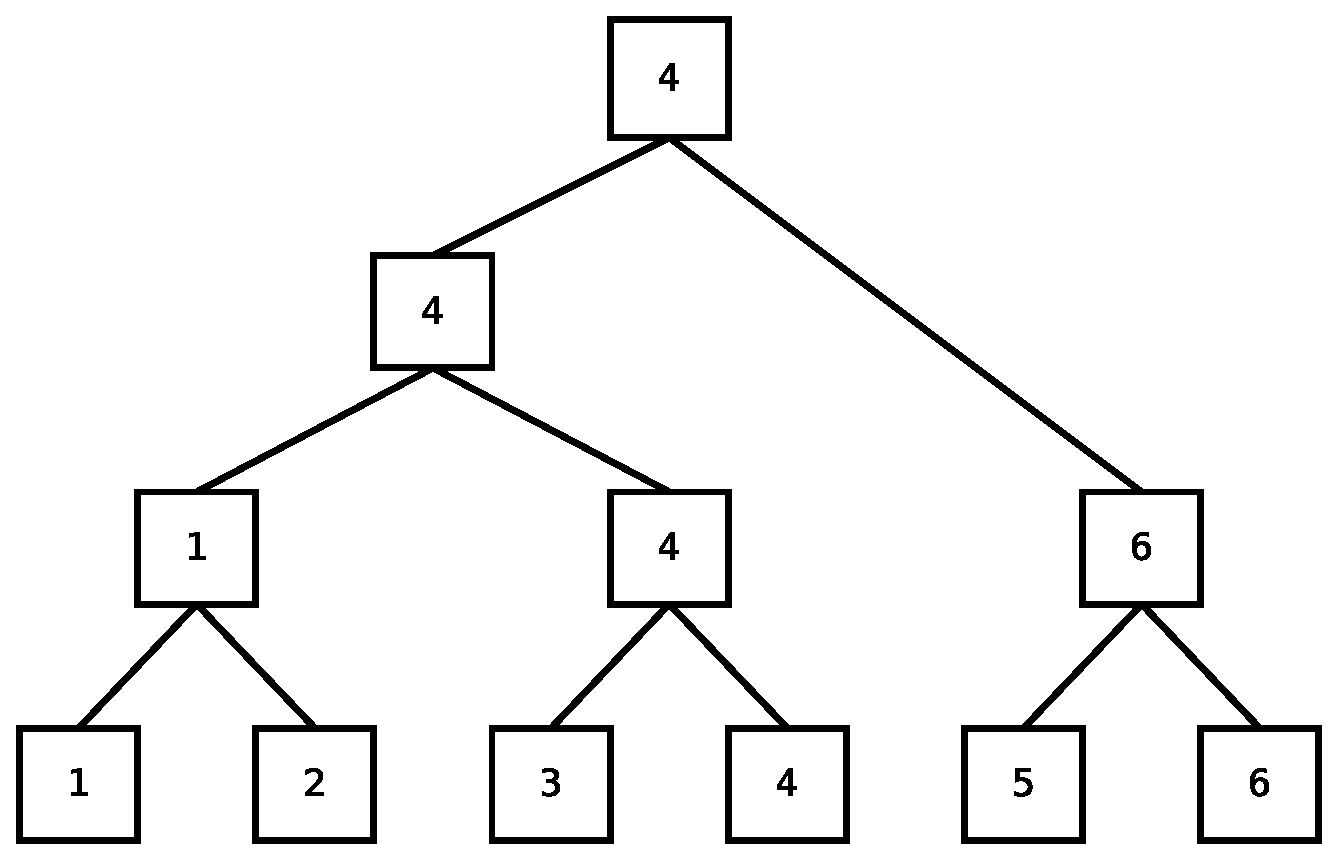
\includegraphics[scale=0.4]{graficos/ArvTorneio1}
	\captionof{figure}{Ilustração de uma árvore de torneio com 6 padrões}
	\label{img:ArvTorneio1}
\end{center}

\begin{center}
	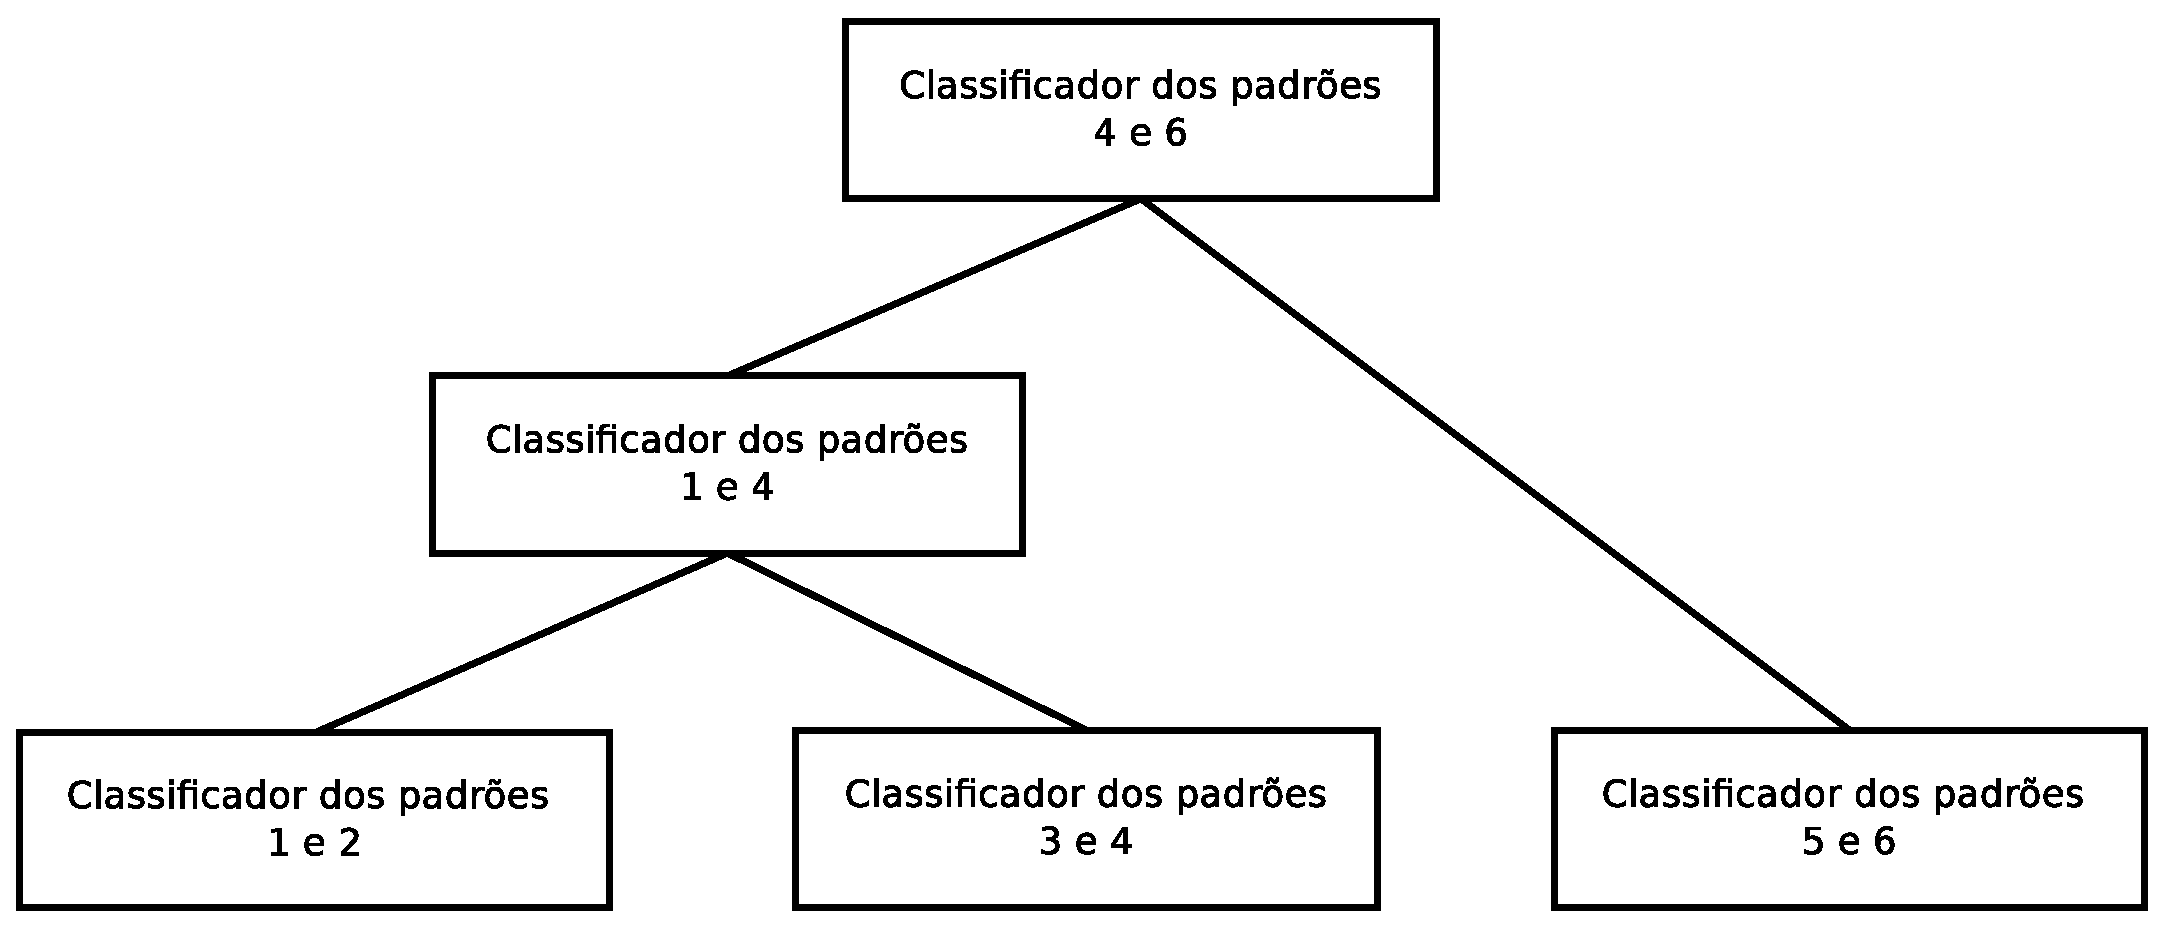
\includegraphics[scale=0.4]{graficos/ArvTorneio2}
	\captionof{figure}{Ilustração de uma árvore de torneio de acordo com os classificadores}
	\label{img:ArvTorneio2}
\end{center}
Depois de obtidos os valores do modelo, é necessário um mecanismo para que um padrão desconhecido possa ser classificado como um dos 7 padrões, ou seja, analisando uma imagem é preciso descobrir qual das 7 expressões ela representa. Para isso, é utilizada uma estrutura chamada árvore de torneio (Hadid, 2005). Por analogia podemos pensar na árvore como a estrutura utilizada em um torneio esportivo e nos padrões como os times do torneio, os times devem se confrontar até que ao final saia o vencedor. Da mesma forma, analisamos os padrões até que ao final se obtenha o padrão ao qual o conjunto submetido pertença.
Na árvore acima, consideramos 7 padrões e o conjunto desconhecido pertencendo ao padrão 7. A quantidade de nós folhas deve ser a quantidade de padrões e a formação dos pares é arbitrária. Analisando o primeiro par, deve ser analisado em qual dos dois padrões o conjunto desconhecido mais se encaixa, ou seja, deve ser analisado de qual lado da reta (gerada pelo modelo quando foram submetidos os padrões 1 e 2)o conjunto desconhecido se encontra. Na figura exemplo, a maioria dos pontos ficaram localizados do mesmo lado da reta que os pontos do padrão 1, por isso esse padrão continuou no próximo nível da árvore e o padrão 2 foi excluído. Esse procedimento ocorre por analogia em todos os pares, até que ao final, quando analisados os padrões 4 e 7, foi definido que o conjunto pertence ao padrão 7.
